% Proof of Canopy: 4-page proposal.
% Build: npm run proposal   (figures.ts, then XeLaTeX via latexmk and latexmkrc in this folder)
% Every measurement below comes from generated/*.tex, which figures.ts writes from the committed data files.
\documentclass[10pt,a4paper]{article}

\usepackage[a4paper, left=17mm, right=17mm, top=15mm, bottom=17mm, footskip=8mm]{geometry}
\usepackage{fontspec}
\setmainfont{InstrumentSans}[
  Path=fonts/, Extension=.ttf,
  UprightFont=*-Regular, BoldFont=*-SemiBold, ItalicFont=*-Italic, BoldItalicFont=*-SemiBoldItalic,
  FontFace={m}{n}{*-Regular}, FontFace={sb}{n}{*-SemiBold}, FontFace={b}{n}{*-Bold}]
\setsansfont{InstrumentSans}[
  Path=fonts/, Extension=.ttf,
  UprightFont=*-Regular, BoldFont=*-SemiBold, ItalicFont=*-Italic, BoldItalicFont=*-SemiBoldItalic]
\setmonofont{IBMPlexMono}[
  Path=fonts/, Extension=.ttf, Scale=0.88,
  UprightFont=*-Regular, BoldFont=*-SemiBold]
\usepackage{amsmath}
\usepackage{xcolor}
\usepackage{tikz}
\usetikzlibrary{arrows.meta, calc, shapes.geometric}
\usepackage{booktabs, tabularx, array}
\usepackage{enumitem}
\usepackage{fancyhdr}
\usepackage{microtype}
\usepackage[hidelinks]{hyperref}

% ------------------------------------------------------------------ palette (same as the website)
\definecolor{ground}{HTML}{F2F3EF}
\definecolor{ink}{HTML}{131712}
\definecolor{ink2}{HTML}{454D44}
\definecolor{ink3}{HTML}{5E665C}
\definecolor{line}{HTML}{D9DCD3}
\definecolor{gridc}{HTML}{E1E3DD}
\definecolor{axisc}{HTML}{9AA197}
\definecolor{canopy}{HTML}{1E4D33}
\definecolor{lost}{HTML}{9A896A}
\definecolor{good}{HTML}{0B7B5C}
\definecolor{warn}{HTML}{B77F14}
\definecolor{critical}{HTML}{A42F1B}
\definecolor{linkc}{HTML}{1F4E9A}
\definecolor{bandbase}{HTML}{E4E7E0}
\definecolor{bandepoch}{HTML}{EDF0EA}
\color{ink}

\newcommand{\mono}[1]{\texttt{#1}}
\newcommand{\link}[2]{\href{#1}{\color{linkc}#2}}
\newcommand{\sect}[2]{\par\vspace{6pt}\noindent{\fontsize{8}{10}\selectfont\ttfamily\color{ink3}#1}\hspace{6pt}{\fontsize{13}{15}\selectfont\bfseries #2}\par\vspace{3pt}}
\newcommand{\figlabel}[1]{\noindent{\small\bfseries #1}\par\vspace{2pt}}
\newcommand{\figcaption}[1]{\par\vspace{3pt}\noindent{\footnotesize\color{ink2}#1}\par}
\newcommand{\sdot}[1]{\tikz[baseline=-0.55ex]\fill[#1] (0,0) circle (2.3pt);}
% results-table cell: status dot, canopy retained -> share of that year's tranche released
\newcommand{\cell}[3]{\sdot{#1}\,\mono{#2}\,{\color{ink3}$\rightarrow$}\,\mono{#3}}

\setlength{\parindent}{0pt}
\setlength{\parskip}{4pt}
\linespread{1.06}
\setlist{nosep, leftmargin=12pt, itemsep=2pt}
\setlength{\tabcolsep}{4pt}

\pagestyle{fancy}
\fancyhf{}
\renewcommand{\headrulewidth}{0pt}
\fancyfoot[L]{\fontsize{7}{9}\selectfont\ttfamily\color{ink3}Proof of Canopy · proofofcanopy.zichengyu.com}
\fancyfoot[R]{\fontsize{7}{9}\selectfont\ttfamily\color{ink3}\thepage\,/\,4}

\tikzset{
  grid/.style={gridc, line width=0.4pt},
  axis/.style={axisc, line width=0.5pt},
  ticklabel/.style={font=\fontsize{5.5}{6.5}\selectfont, text=ink3, inner sep=1pt},
  sidelabel/.style={anchor=west, font=\fontsize{5.5}{6.5}\selectfont, text=ink2, inner sep=1pt},
  baseline/.style={ink2, dash pattern=on 1pt off 1.6pt, line width=0.5pt},
  threshold/.style={ink, dash pattern=on 3pt off 2pt, line width=0.6pt},
  fire/.style={critical, line width=0.8pt},
  series/.style={ink2, line width=0.55pt, line join=round},
  basepoint/.style={circle, draw=ink2, fill=white, line width=0.5pt, inner sep=0pt, minimum size=3.4pt},
  scored/.style={circle, draw=white, line width=0.4pt, inner sep=0pt, minimum size=4.8pt},
  rejected/.style={circle, draw=critical, fill=white, line width=0.6pt, inner sep=0pt, minimum size=6pt},
  annot/.style={font=\fontsize{5.5}{6.6}\selectfont, text=ink, inner sep=1pt, fill=white, fill opacity=0.85, text opacity=1},
  epochlabel/.style={anchor=north, font=\fontsize{5.5}{6.5}\selectfont, text=ink, inner sep=1pt},
  rulepoint/.style={draw=white, line width=0.3pt, inner sep=0pt, minimum size=4.8pt},
}

% Generated by docs/proposal/figures.ts. Do not edit.
\newcommand{\SeriesMonths}{93}
\newcommand{\SeriesFrom}{\mbox{2019-01}}
\newcommand{\SeriesTo}{\mbox{2026-09}}
\newcommand{\FireMonth}{\mbox{2021-08}}
\newcommand{\FireFirms}{15}
\newcommand{\FireFirst}{\mbox{2021-08-01}}
\newcommand{\FireLast}{\mbox{2021-08-02}}
\newcommand{\FireDnbr}{0.33}
\newcommand{\FireBefore}{0.83}
\newcommand{\FireAfter}{0.00}
\newcommand{\NovoFireMonth}{\mbox{2024-09}}
\newcommand{\NovoFireFirms}{5}
\newcommand{\NovoFireDnbr}{0.13}
\newcommand{\SmokeBefore}{0.79}
\newcommand{\SmokeAfter}{0.01}
\newcommand{\SmokeNbr}{0.54}
\newcommand{\FalseClaim}{94\%}
\newcommand{\FalseRecompute}{14.49\%}
\newcommand{\ReleasedHealthy}{0.002995}
\newcommand{\ReleasedDegraded}{0.001798}
\newcommand{\ReleasedBurned}{0.000000}
\newcommand{\ReturnedTotal}{0.004207}
\newcommand{\BaselineHealthy}{0.99}
\newcommand{\MinHealthy}{99.8\%}
\newcommand{\MaxHealthy}{100\%}
\newcommand{\BaselineDegraded}{0.97}
\newcommand{\MinDegraded}{81.7\%}
\newcommand{\MaxDegraded}{100\%}
\newcommand{\BaselineBurned}{0.92}
\newcommand{\MinBurned}{14.5\%}
\newcommand{\MaxBurned}{50.9\%}

\newcommand{\ResultsRows}{%
\textbf{Yedigöller} {\color{ink3}\scriptsize healthy} & \cell{good}{100\%}{100\%} & \cell{good}{100\%}{100\%} & \cell{good}{100\%}{100\%} & \cell{good}{100\%}{100\%} & \cell{good}{99.8\%}{99.4\%} & \mono{0.002995} \\
\textbf{Novo Progresso} {\color{ink3}\scriptsize degraded} & \cell{good}{100\%}{100\%} & \cell{warn}{81.7\%}{38.9\%} & \cell{warn}{86.9\%}{56.4\%} & \cell{warn}{86.1\%}{53.8\%} & \cell{warn}{89.4\%}{64.6\%} & \mono{0.001798} \\
\textbf{Manavgat} {\color{ink3}\scriptsize burned} & \cell{critical}{16.2\%}{0\%} & \cell{critical}{14.5\%}{0\%} & \cell{critical}{26.6\%}{0\%} & \cell{critical}{47.5\%}{0\%} & \cell{critical}{50.9\%}{0\%} & \mono{0.000000} \\
}


\begin{document}

% =================================================================================== page 1
{\fontsize{7.5}{9}\selectfont\ttfamily\color{ink3}IEEE CLIMATECHAIN GLOBAL HACKATHON · TRACK: CARBON MARKETS \& EMISSIONS TRANSPARENCY}\par
\vspace{6pt}
{\fontsize{30}{32}\selectfont\bfseries Proof of Canopy}\par
\vspace{4pt}
{\fontsize{14}{17}\selectfont\color{ink2}Afforestation funding, released only while the forest is still standing.}\par
\vspace{6pt}
{\footnotesize
\begin{tabularx}{\textwidth}{@{}l@{\hspace{10pt}}X@{}}
Live site & \link{https://proofofcanopy.zichengyu.com}{proofofcanopy.zichengyu.com} (reads Base Sepolia live)\\
Code & \link{https://github.com/zicheng-yu/proof-of-canopy}{github.com/zicheng-yu/proof-of-canopy}\\
Video & \link{https://proofofcanopy.zichengyu.com/video/}{proofofcanopy.zichengyu.com/video} (3:26, recorded live on Base Sepolia)\\
\end{tabularx}}

\vspace{6pt}
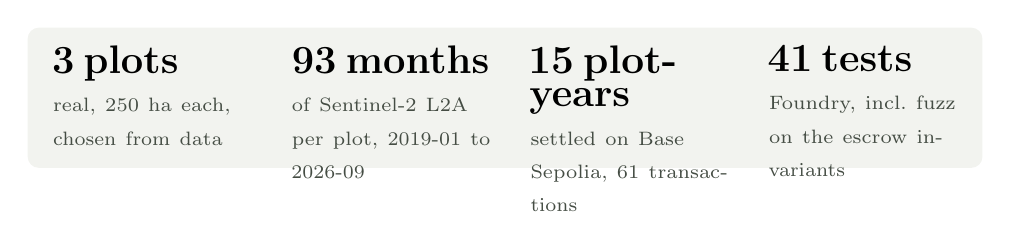
\begin{tikzpicture}
  \fill[ground, rounded corners=4pt] (0,0) rectangle (\textwidth,1.78);
  \foreach \i/\big/\small in {
      0/{3 plots}/{real, 250 ha each, chosen from data},
      1/{\SeriesMonths\ months}/{of Sentinel-2 L2A per plot, \SeriesFrom\ to \SeriesTo},
      2/{15 plot-years}/{settled on Base Sepolia, 61 transactions},
      3/{41 tests}/{Foundry, incl.\ fuzz on the escrow invariants}} {
    \node[anchor=north west, text width=0.25\textwidth-14pt, align=left, inner sep=0pt]
      at ({\i*0.25\textwidth+9pt}, 1.56) {{\fontsize{15}{17}\selectfont\bfseries \big}\\[2pt]{\fontsize{7.5}{9}\selectfont\color{ink2}\small}};
  }
\end{tikzpicture}

\sect{01}{The problem}
Forest carbon projects promise decades of storage, but the money and the credits often move once, after a single
verification near planting. If the trees burn or are cleared in year two, nothing in the payment flow reacts, and
whoever certified the plot carries no consequence for having been wrong. Buyers end up paying for a promise rather
than for forest that is still there.

\sect{02}{What Proof of Canopy does}
Funding sits in an on-chain escrow and is released one year at a time, in proportion to how much of the plot's
2019--2020 canopy Sentinel-2 still sees. At or below a threshold fixed when the project registers (here
$T = 70\%$), that year's tranche is frozen; a plot that recovers still earns its later tranches, and whatever stayed
frozen returns to the funder after the last year. The survival figure is reported by a verifier who stakes on every
claim. Anyone can challenge a claim inside a window by posting a bond, and whoever turns out to be wrong loses
their deposit: half to the other side, half burned.

\vspace{2pt}
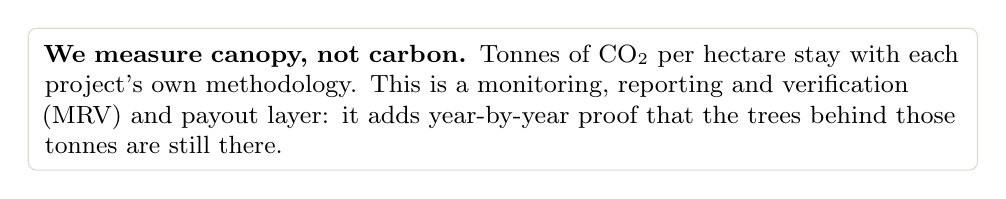
\begin{tikzpicture}
  \node[draw=line, fill=white, rounded corners=3pt, text width=\textwidth-14pt, inner sep=6pt, align=left, font=\small]
    {\textbf{We measure canopy, not carbon.} Tonnes of CO\textsubscript{2} per hectare stay with each project's own
     methodology. This is a monitoring, reporting and verification (MRV) and payout layer: it adds year-by-year proof
     that the trees behind those tonnes are still there.};
\end{tikzpicture}

\sect{03}{Five years, three real plots}
\vspace{-1pt}
{\footnotesize
\renewcommand{\arraystretch}{1.25}
\begin{tabularx}{\textwidth}{@{}X*{5}{c}r@{}}
\toprule
\textbf{Plot} & \textbf{2021 (E0)} & \textbf{2022 (E1)} & \textbf{2023 (E2)} & \textbf{2024 (E3)} & \textbf{2025 (E4)} & \textbf{Released, ETH}\\
\midrule
\ResultsRows
\bottomrule
\end{tabularx}}
\figcaption{Each cell: canopy retained against the 2019--2020 baseline $\rightarrow$ share of that year's tranche released,
as settled on chain. Tranches are 10/15/20/25/30\% of 0.003 ETH per project (testnet amounts).
\sdot{good}\,holding ($\geq 95\%$) \quad \sdot{warn}\,degrading \quad \sdot{critical}\,at or below $T$, tranche frozen.
After the last epoch the funder reclaimed the \ReturnedTotal\ ETH that stayed frozen.}

\sect{04}{What is built and running}
\begin{itemize}
  \item \textbf{Satellite evidence pipeline} (\mono{oracle/}): picks plots from a grid scan, fetches monthly Sentinel-2
        statistics from the Copernicus Data Space and NASA FIRMS fire detections, and writes one evidence file per
        plot-year that cites the monthly series by hash.
  \item \textbf{Three Solidity contracts on Base Sepolia}, sources verified on Sourcify: \mono{ProjectRegistry},
        \mono{SurvivalOracle}, \mono{MilestoneEscrow}. The full story ran on them: registration, a refused double
        registration, funding, all 15 plot-years settled, a staged false claim challenged and slashed, frozen money
        reclaimed and earned money withdrawn.
  \item \textbf{A read-only website} that rebuilds every number from contract events and lets anyone re-hash the
        evidence and recompute survival in the browser, with the same code the oracle runs.
  \item \textbf{Escrow invariants under fuzzing:} tranches always sum to the escrowed amount, a higher survival never
        releases less, and every wei of a settled tranche is either released or frozen.
\end{itemize}

\newpage
% =================================================================================== page 2
\sect{05}{Architecture}
\vspace{2pt}
\begin{tikzpicture}[x=1cm, y=1cm,
    panel/.style={fill=ground, rounded corners=4pt},
    plabel/.style={anchor=north west, font=\fontsize{6}{7}\selectfont\ttfamily, text=ink3, inner sep=0pt},
    box/.style={anchor=north west, draw=line, fill=white, rounded corners=2.5pt, align=left, inner sep=4pt,
                font=\fontsize{6.8}{8.4}\selectfont},
    cbox/.style={box, draw=ink, line width=0.6pt},
    arr/.style={-{Stealth[length=4pt, width=3.2pt]}, line width=0.6pt, ink2},
    lab/.style={font=\fontsize{5.8}{7}\selectfont, text=ink2, inner sep=1pt}]

  % off-chain
  \fill[panel] (0,6.35) rectangle (17.0,9.95);
  \node[plabel] at (0.2,9.77) {OFF-CHAIN · REPRODUCIBLE FROM PUBLISHED FILES};
  \node[box, text width=3.2cm] (s2) at (0.2,9.42) {\textbf{Sentinel-2 L2A}\\Copernicus Data Space, Statistical API · 10\,m · least-cloudy scene per month};
  \node[box, text width=3.2cm] (firms) at (0.2,7.8) {\textbf{NASA FIRMS}\\VIIRS active-fire detections around the plot};
  \node[box, text width=6.0cm] (orc) at (4.2,9.42) {\textbf{Oracle} \mono{oracle/run.ts} · method in \mono{shared/method.ts}\\
      clouds, shadow and snow masked per pixel (SCL)\\
      NDVI histogram per month; canopy = pixels with NDVI $\geq 0.5$\\
      year score = greenest cloud-free Aug--Oct month\\
      $s$ = score / median of 2019--20 · fires: dNBR + FIRMS};
  \node[box, text width=4.9cm] (ev) at (11.05,9.42) {\textbf{Published evidence}, written once\\
      \mono{plots/<id>.geojson}\quad boundary\\
      \mono{series/<id>.json}\quad \SeriesMonths\ monthly histograms\\
      \mono{attestations/<id>/epoch-n.json}\\
      \quad survival, scored months, \mono{seriesHash}};
  \draw[arr] (s2.east) -- (s2.east -| orc.west);
  \draw[arr] (firms.east) -- (firms.east -| orc.west);
  \draw[arr] (orc.east |- ev.west) -- (ev.west);

  % on-chain
  \fill[panel] (0,2.55) rectangle (17.0,5.95);
  \node[plabel] at (0.2,5.77) {ON-CHAIN · BASE SEPOLIA · HOLDS IDENTITY, MONEY AND STAKED CLAIMS};
  \node[cbox, text width=4.5cm] (reg) at (0.2,5.4) {\textbf{ProjectRegistry}\\
      one identity per plot: \mono{plotHash} = keccak256 of the boundary bytes, plus the H3 cells it covers
      (res 9); a cell can belong to one project only\\[2pt]
      {\color{ink3}developer registers · threshold $T$ fixed here}};
  \node[cbox, text width=5.8cm] (orac) at (5.45,5.4) {\textbf{SurvivalOracle}\\
      verifier stakes, attests \mono{survivalBps} and \mono{evidenceHash} for one plot-year; anyone may challenge in
      the window with a bond\\[2pt]
      {\color{ink3}arbiter resolves · loser's deposit 50\% to winner, 50\% burned}};
  \node[cbox, text width=4.5cm] (esc) at (12.1,5.4) {\textbf{MilestoneEscrow}\\
      funder escrows once; each final year releases tranche $\times f(s)$ and freezes the rest; frozen funds go back
      after the last year\\[2pt]
      {\color{ink3}pull payments · releases read only final claims}};
  \draw[arr] (reg.east) -- (orac.west);
  \draw[arr] (orac.east) -- (esc.west);
  \coordinate (va) at ($(ev.south west)+(0.3,0)$);
  \draw[arr] (va) -- (va |- orac.north);
  \node[lab, anchor=west] at ($(va)+(0.08,-0.32)$) {verifier attests \mono{survivalBps} + keccak256(evidence)};

  % website
  \fill[panel] (0,0) rectangle (17.0,2.15);
  \node[plabel] at (0.2,1.97) {READ-ONLY WEBSITE · NO WALLET, NO SERVER};
  \node[box, text width=7.6cm] (pages) at (0.2,1.65) {\textbf{Overview and plot pages}\\
      every number rebuilt in the browser from contract events, polled every 3\,s: escrow, releases, claims,
      disputes, each with its transaction};
  \node[box, text width=7.95cm] (ver) at (8.65,1.65) {\textbf{Verify page}\\
      fetch the published files, keccak256 their bytes and compare with the chain; recompute survival from the
      series with the oracle's own \mono{shared/method.ts}};
  \draw[arr] (6.4,2.55) -- (6.4,1.65);
  \node[lab, anchor=west] at (6.48,2.35) {contract events};
  \draw[arr] (9.4,2.55) -- (9.4,1.65);
  \node[lab, anchor=west] at (9.48,2.35) {stored hashes, cells, \mono{survivalBps}};
  \draw[arr] (ev.east) -- (17.25,0 |- ev.east) |- node[lab, rotate=90, anchor=south, pos=0.25] {fetch and re-hash} (ver.east);
\end{tikzpicture}
\figcaption{The measurement stays off chain and can be rerun by anyone from the published files; the chain holds what no
single party should hold (the plot's identity, the money, and a public, staked record of who claimed what); the website
only reads.}

\vspace{6pt}
\begin{minipage}[t]{0.5\textwidth}
\figlabel{Life of one claim}
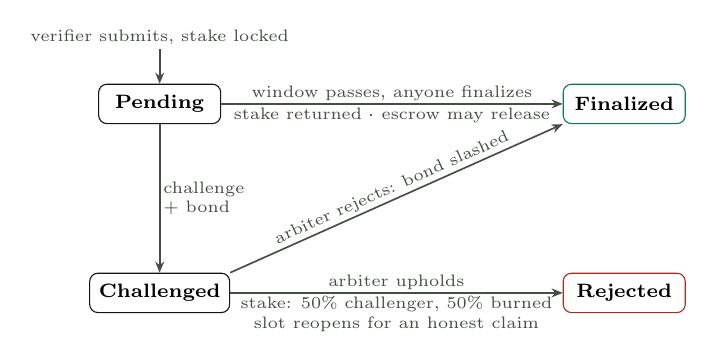
\begin{tikzpicture}[x=1cm, y=1cm,
    st/.style={draw=ink, fill=white, rounded corners=3pt, font=\fontsize{7}{8}\selectfont\bfseries, minimum width=1.55cm, minimum height=0.5cm},
    arr/.style={-{Stealth[length=4pt, width=3.2pt]}, line width=0.6pt, ink2},
    lab/.style={font=\fontsize{5.8}{7}\selectfont, text=ink2, inner sep=1pt, align=center}]
  \node[st] (p) at (1.0,2.75) {Pending};
  \node[st, draw=good] (f) at (6.9,2.75) {Finalized};
  \node[st] (c) at (1.0,0.35) {Challenged};
  \node[st, draw=critical] (r) at (6.9,0.35) {Rejected};
  \draw[arr] (1.0,3.45) node[lab, above] {verifier submits, stake locked} -- (p.north);
  \draw[arr] (p) -- node[lab, above] {window passes, anyone finalizes} node[lab, below] {stake returned · escrow may release} (f);
  \draw[arr] (p) -- node[lab, right, align=left] {challenge\\+ bond} (c);
  \draw[arr] (c) -- node[lab, above, pos=0.5] {arbiter upholds} node[lab, below] {stake: 50\% challenger, 50\% burned\\slot reopens for an honest claim} (r);
  \draw[arr] (c.north east) -- node[lab, sloped, above, pos=0.5] {arbiter rejects: bond slashed} (f.south west);
\end{tikzpicture}
\end{minipage}%
\begin{minipage}[t]{0.5\textwidth}
\figlabel{Release rule, with all 15 settled plot-years}
\hspace*{0.5cm}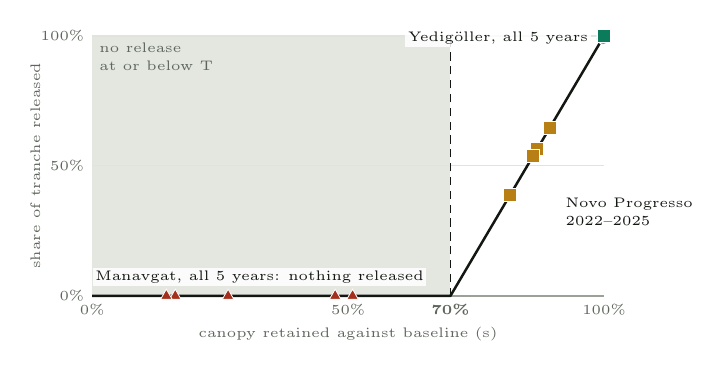
\begin{tikzpicture}[x=1cm,y=1cm]
\fill[bandbase] (0,0) rectangle (4.550,3.300);
\node[ticklabel, anchor=north west, align=left] at (0.05,3.250) {no release\\at or below T};
\draw[grid] (0,1.650) -- (6.500,1.650);
\draw[grid] (0,3.300) -- (6.500,3.300);
\draw[axis] (0,0) -- (6.500,0);
\node[ticklabel, anchor=east] at (-0.06,0.000) {0\%};
\node[ticklabel, anchor=north] at (0.000,-0.06) {0\%};
\node[ticklabel, anchor=east] at (-0.06,1.650) {50\%};
\node[ticklabel, anchor=north] at (3.250,-0.06) {50\%};
\node[ticklabel, anchor=east] at (-0.06,3.300) {100\%};
\node[ticklabel, anchor=north] at (6.500,-0.06) {100\%};
\node[ticklabel, anchor=north, font=\tiny\bfseries] at (4.550,-0.06) {70\%};
\draw[threshold] (4.550,0) -- (4.550,3.300);
\draw[ink, line width=0.9pt, line join=round] (0,0) -- (4.550,0) -- (6.500,3.300);
\node[rulepoint, circle, fill=good] at (6.500,3.300) {};
\node[rulepoint, circle, fill=good] at (6.500,3.300) {};
\node[rulepoint, circle, fill=good] at (6.500,3.300) {};
\node[rulepoint, circle, fill=good] at (6.500,3.300) {};
\node[rulepoint, circle, fill=good] at (6.489,3.281) {};
\node[rulepoint, rectangle, fill=good] at (6.500,3.300) {};
\node[rulepoint, rectangle, fill=warn] at (5.309,1.285) {};
\node[rulepoint, rectangle, fill=warn] at (5.650,1.862) {};
\node[rulepoint, rectangle, fill=warn] at (5.598,1.774) {};
\node[rulepoint, rectangle, fill=warn] at (5.810,2.132) {};
\node[rulepoint, regular polygon, regular polygon sides=3, fill=critical] at (1.055,0.000) {};
\node[rulepoint, regular polygon, regular polygon sides=3, fill=critical] at (0.942,0.000) {};
\node[rulepoint, regular polygon, regular polygon sides=3, fill=critical] at (1.726,0.000) {};
\node[rulepoint, regular polygon, regular polygon sides=3, fill=critical] at (3.086,0.000) {};
\node[rulepoint, regular polygon, regular polygon sides=3, fill=critical] at (3.307,0.000) {};
\node[annot, anchor=east] at (6.340,3.280) {Yedigöller, all 5 years};
\node[annot, anchor=north west, align=left] at (5.970,1.285) {Novo Progresso\\2022--2025};
\node[annot, anchor=south] at (2.125,0.12) {Manavgat, all 5 years: nothing released};
\node[ticklabel, anchor=north] at (3.250,-0.36) {canopy retained against baseline (s)};
\node[ticklabel, anchor=south, rotate=90] at (-0.62,1.650) {share of tranche released};
\end{tikzpicture}

\par\vspace{1pt}
{\footnotesize\color{ink2}$f(s) = \operatorname{clamp}\!\big((s - T)/(1 - T),\, 0,\, 1\big)$, $T = 70\%$.\\
\tikz\node[circle, fill=ink3, inner sep=0, minimum size=4pt]{};\,Yedigöller
\ \tikz\node[rectangle, fill=ink3, inner sep=0, minimum size=4pt]{};\,Novo Progresso
\ \tikz\node[regular polygon, regular polygon sides=3, fill=ink3, inner sep=0, minimum size=5pt]{};\,Manavgat}
\end{minipage}



\sect{06}{Verify it yourself}
The website's Verify page runs four checks in the browser for any attestation. For the staged false claim (attestation
\#15, ``Manavgat recovered to \FalseClaim\ in 2022''), the file is genuine but the number is not:

{\footnotesize
\renewcommand{\arraystretch}{1.2}
\begin{tabularx}{\textwidth}{@{}>{\raggedright\arraybackslash}p{4.1cm}>{\raggedright\arraybackslash}X>{\raggedright\arraybackslash}p{4.4cm}@{}}
\toprule
\textbf{Check} & \textbf{What the browser does} & \textbf{Attestation \#15}\\
\midrule
Evidence file matches the claim & keccak256 of the published file's bytes vs.\ \mono{evidenceHash} on chain & \sdot{good}\,match\\
Boundary matches the plot & keccak256 of the GeoJSON bytes vs.\ \mono{plotHash} & \sdot{good}\,match\\
Cells match the boundary & recompute the H3 res-9 cells with h3-js vs.\ \mono{cellsOf} & \sdot{good}\,22 of 22 identical\\
Survival follows from the satellite series & check \mono{seriesHash}, rerun \mono{shared/method.ts} on the series vs.\ \mono{survivalBps} & \sdot{critical}\,recomputed \FalseRecompute, claimed \FalseClaim: mismatch\\
\bottomrule
\end{tabularx}}


\newpage
% =================================================================================== page 3
\sect{07}{Measuring canopy}
\begin{enumerate}[leftmargin=14pt]
  \item \textbf{Pick plots from data, not by eye.} \mono{oracle/scan.ts} scores a grid of 250\,ha squares by
        late-season canopy in a baseline and a test year. For the burned plot the grid is centred on the densest cluster of
        FIRMS detections during the July--August 2021 Manavgat fire.
  \item \textbf{Fetch the series.} One Statistical API request per plot returns \SeriesMonths\ months
        (\SeriesFrom\ to \SeriesTo) of Sentinel-2 L2A at 10\,m: the least cloudy scene of each month, clouds,
        shadow, cirrus and snow masked per pixel, and a 40-bin NDVI histogram. Canopy fraction = share of cloud-free
        pixels with NDVI $\geq 0.5$; months under 60\% cloud-free are not used.
  \item \textbf{Score each year on its greenest Aug--Oct month}, against the median of 2019 and 2020. Clouds, haze and
        smoke only ever lower NDVI, so the maximum is the reading least contaminated by them, while real canopy loss
        lowers every month. Survival $s$ is the ratio, capped at 1, in basis points.
  \item \textbf{Write evidence once.} Each plot-year file carries the baseline, the observed value, the months used, $s$,
        and \mono{seriesHash} = keccak256 of the series file. The chain stores keccak256 of the evidence file itself.
\end{enumerate}

\vspace{4pt}
\figlabel{Yedigöller \textmd{\color{ink2}· Bolu, Türkiye · national park forest}}
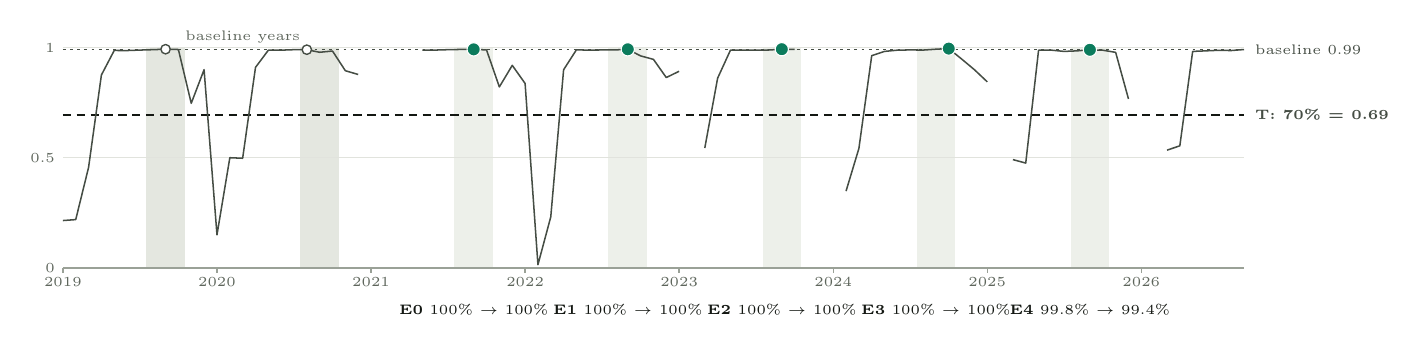
\begin{tikzpicture}[x=1cm,y=1cm]
\fill[bandbase] (1.060,0) rectangle (1.549,2.800);
\fill[bandbase] (3.016,0) rectangle (3.505,2.800);
\fill[bandepoch] (4.973,0) rectangle (5.462,2.800);
\fill[bandepoch] (6.929,0) rectangle (7.418,2.800);
\fill[bandepoch] (8.886,0) rectangle (9.375,2.800);
\fill[bandepoch] (10.842,0) rectangle (11.332,2.800);
\fill[bandepoch] (12.799,0) rectangle (13.288,2.800);
\draw[grid] (0,1.400) -- (15.000,1.400);
\draw[grid] (0,2.800) -- (15.000,2.800);
\draw[axis] (0,0) -- (15.000,0);
\node[ticklabel, anchor=east] at (-0.06,0.000) {0};
\node[ticklabel, anchor=east] at (-0.06,1.400) {0.5};
\node[ticklabel, anchor=east] at (-0.06,2.800) {1};
\draw[axis] (0.000,0) -- (0.000,-0.06);
\node[ticklabel, anchor=north] at (0.000,-0.08) {2019};
\draw[axis] (1.957,0) -- (1.957,-0.06);
\node[ticklabel, anchor=north] at (1.957,-0.08) {2020};
\draw[axis] (3.913,0) -- (3.913,-0.06);
\node[ticklabel, anchor=north] at (3.913,-0.08) {2021};
\draw[axis] (5.870,0) -- (5.870,-0.06);
\node[ticklabel, anchor=north] at (5.870,-0.08) {2022};
\draw[axis] (7.826,0) -- (7.826,-0.06);
\node[ticklabel, anchor=north] at (7.826,-0.08) {2023};
\draw[axis] (9.783,0) -- (9.783,-0.06);
\node[ticklabel, anchor=north] at (9.783,-0.08) {2024};
\draw[axis] (11.739,0) -- (11.739,-0.06);
\node[ticklabel, anchor=north] at (11.739,-0.08) {2025};
\draw[axis] (13.696,0) -- (13.696,-0.06);
\node[ticklabel, anchor=north] at (13.696,-0.08) {2026};
\node[ticklabel, anchor=south] at (2.283,2.820) {baseline years};
\draw[baseline] (0,2.777) -- (15.000,2.777);
\draw[threshold] (0,1.944) -- (15.000,1.944);
\node[sidelabel] at (15.100,2.777) {baseline 0.99};
\node[sidelabel, font=\tiny\bfseries] at (15.100,1.944) {T: 70\% = 0.69};
\draw[series] (0.000,0.604) -- (0.163,0.616) -- (0.326,1.278) -- (0.489,2.452) -- (0.652,2.764) -- (0.815,2.763) -- (0.978,2.769) -- (1.141,2.774) -- (1.304,2.780) -- (1.467,2.776) -- (1.630,2.093) -- (1.793,2.520) -- (1.957,0.422) -- (2.120,1.402) -- (2.283,1.395) -- (2.446,2.549) -- (2.609,2.767) -- (2.772,2.768) -- (2.935,2.774) -- (3.098,2.774) -- (3.261,2.741) -- (3.424,2.757) -- (3.587,2.507) -- (3.750,2.459);
\draw[series] (4.239,1.603);
\draw[series] (4.565,2.768) -- (4.728,2.769) -- (4.891,2.774) -- (5.054,2.777) -- (5.217,2.778) -- (5.380,2.771) -- (5.543,2.301) -- (5.707,2.575) -- (5.870,2.345) -- (6.033,0.043) -- (6.196,0.651) -- (6.359,2.519) -- (6.522,2.773) -- (6.685,2.767) -- (6.848,2.771) -- (7.011,2.771) -- (7.174,2.779) -- (7.337,2.695) -- (7.500,2.651) -- (7.663,2.420) -- (7.826,2.500);
\draw[series] (8.152,1.525) -- (8.315,2.412) -- (8.478,2.768) -- (8.641,2.769) -- (8.804,2.768) -- (8.967,2.770) -- (9.130,2.780) -- (9.293,2.777);
\draw[series] (9.620,2.567);
\draw[series] (9.946,0.978) -- (10.109,1.519) -- (10.272,2.698) -- (10.435,2.752) -- (10.598,2.768) -- (10.761,2.771) -- (10.924,2.769) -- (11.087,2.780) -- (11.250,2.788) -- (11.413,2.656) -- (11.576,2.520) -- (11.739,2.366);
\draw[series] (12.065,1.378) -- (12.228,1.334) -- (12.391,2.767) -- (12.554,2.768) -- (12.717,2.752) -- (12.880,2.759) -- (13.043,2.773) -- (13.207,2.767) -- (13.370,2.740) -- (13.533,2.148);
\draw[series] (14.022,1.498) -- (14.185,1.553) -- (14.348,2.752) -- (14.511,2.759) -- (14.674,2.766) -- (14.837,2.763) -- (15.000,2.776);
\node[basepoint] at (1.304,2.780) {};
\node[basepoint] at (3.098,2.774) {};
\node[scored, fill=good] at (5.217,2.778) {};
\node[scored, fill=good] at (7.174,2.779) {};
\node[scored, fill=good] at (9.130,2.780) {};
\node[scored, fill=good] at (11.250,2.788) {};
\node[scored, fill=good] at (13.043,2.773) {};
\node[epochlabel] at (5.217,-0.42) {\textbf{E0} 100\% $\rightarrow$ 100\%};
\node[epochlabel] at (7.174,-0.42) {\textbf{E1} 100\% $\rightarrow$ 100\%};
\node[epochlabel] at (9.130,-0.42) {\textbf{E2} 100\% $\rightarrow$ 100\%};
\node[epochlabel] at (11.087,-0.42) {\textbf{E3} 100\% $\rightarrow$ 100\%};
\node[epochlabel] at (13.043,-0.42) {\textbf{E4} 99.8\% $\rightarrow$ 99.4\%};
\end{tikzpicture}


\vspace{4pt}
\figlabel{Novo Progresso \textmd{\color{ink2}· Pará, Brazil · deforestation arc}}
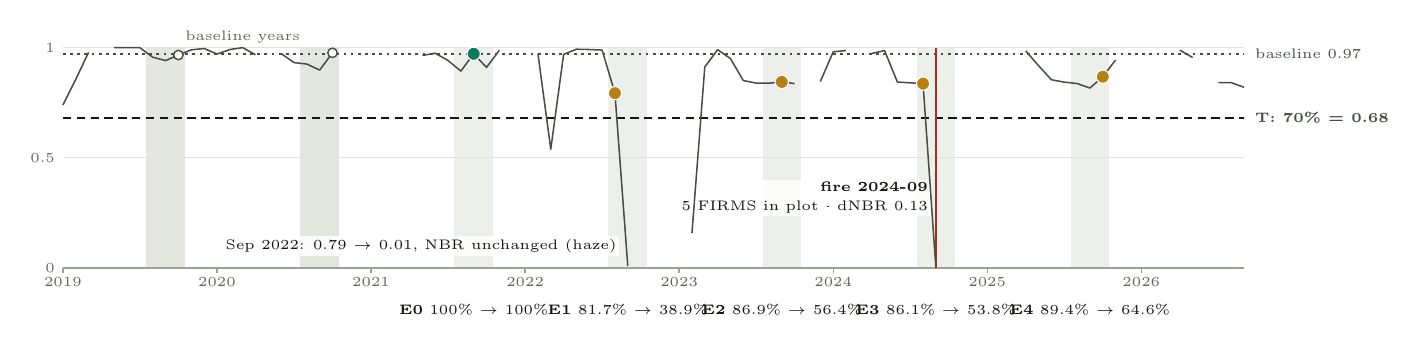
\begin{tikzpicture}[x=1cm,y=1cm]
\fill[bandbase] (1.060,0) rectangle (1.549,2.800);
\fill[bandbase] (3.016,0) rectangle (3.505,2.800);
\fill[bandepoch] (4.973,0) rectangle (5.462,2.800);
\fill[bandepoch] (6.929,0) rectangle (7.418,2.800);
\fill[bandepoch] (8.886,0) rectangle (9.375,2.800);
\fill[bandepoch] (10.842,0) rectangle (11.332,2.800);
\fill[bandepoch] (12.799,0) rectangle (13.288,2.800);
\draw[grid] (0,1.400) -- (15.000,1.400);
\draw[grid] (0,2.800) -- (15.000,2.800);
\draw[axis] (0,0) -- (15.000,0);
\node[ticklabel, anchor=east] at (-0.06,0.000) {0};
\node[ticklabel, anchor=east] at (-0.06,1.400) {0.5};
\node[ticklabel, anchor=east] at (-0.06,2.800) {1};
\draw[axis] (0.000,0) -- (0.000,-0.06);
\node[ticklabel, anchor=north] at (0.000,-0.08) {2019};
\draw[axis] (1.957,0) -- (1.957,-0.06);
\node[ticklabel, anchor=north] at (1.957,-0.08) {2020};
\draw[axis] (3.913,0) -- (3.913,-0.06);
\node[ticklabel, anchor=north] at (3.913,-0.08) {2021};
\draw[axis] (5.870,0) -- (5.870,-0.06);
\node[ticklabel, anchor=north] at (5.870,-0.08) {2022};
\draw[axis] (7.826,0) -- (7.826,-0.06);
\node[ticklabel, anchor=north] at (7.826,-0.08) {2023};
\draw[axis] (9.783,0) -- (9.783,-0.06);
\node[ticklabel, anchor=north] at (9.783,-0.08) {2024};
\draw[axis] (11.739,0) -- (11.739,-0.06);
\node[ticklabel, anchor=north] at (11.739,-0.08) {2025};
\draw[axis] (13.696,0) -- (13.696,-0.06);
\node[ticklabel, anchor=north] at (13.696,-0.08) {2026};
\node[ticklabel, anchor=south] at (2.283,2.820) {baseline years};
\draw[baseline] (0,2.720) -- (15.000,2.720);
\draw[threshold] (0,1.904) -- (15.000,1.904);
\node[sidelabel] at (15.100,2.720) {baseline 0.97};
\node[sidelabel, font=\tiny\bfseries] at (15.100,1.904) {T: 70\% = 0.68};
\draw[fire] (11.087,0) -- (11.087,2.800);
\node[annot, anchor=east, align=right] at (11.027,0.896) {\textbf{fire 2024-09}\\5 FIRMS in plot · dNBR 0.13};
\draw[series] (0.000,2.071) -- (0.163,2.396) -- (0.326,2.740);
\draw[series] (0.652,2.800) -- (0.815,2.800) -- (0.978,2.799) -- (1.141,2.678) -- (1.304,2.636) -- (1.467,2.706) -- (1.630,2.772) -- (1.793,2.789) -- (1.957,2.718) -- (2.120,2.776) -- (2.283,2.800) -- (2.446,2.710);
\draw[series] (2.772,2.725) -- (2.935,2.610) -- (3.098,2.591) -- (3.261,2.515) -- (3.424,2.734);
\draw[series] (3.913,2.651);
\draw[series] (4.565,2.701) -- (4.728,2.729) -- (4.891,2.637) -- (5.054,2.502) -- (5.217,2.722) -- (5.380,2.549) -- (5.543,2.766);
\draw[series] (6.033,2.724) -- (6.196,1.510) -- (6.359,2.714) -- (6.522,2.780) -- (6.685,2.776) -- (6.848,2.769) -- (7.011,2.222) -- (7.174,0.027);
\draw[series] (7.989,0.444) -- (8.152,2.554) -- (8.315,2.774) -- (8.478,2.661) -- (8.641,2.382) -- (8.804,2.350) -- (8.967,2.348) -- (9.130,2.365) -- (9.293,2.343);
\draw[series] (9.620,2.370) -- (9.783,2.747) -- (9.946,2.763);
\draw[series] (10.272,2.726) -- (10.435,2.762) -- (10.598,2.363) -- (10.761,2.353) -- (10.924,2.343) -- (11.087,0.002);
\draw[series] (12.228,2.758) -- (12.391,2.571) -- (12.554,2.392) -- (12.717,2.362) -- (12.880,2.344) -- (13.043,2.287) -- (13.207,2.431) -- (13.370,2.644);
\draw[series] (14.185,2.768) -- (14.348,2.674);
\draw[series] (14.674,2.355) -- (14.837,2.356) -- (15.000,2.296);
\node[basepoint] at (1.467,2.706) {};
\node[basepoint] at (3.424,2.734) {};
\node[scored, fill=good] at (5.217,2.722) {};
\node[scored, fill=warn] at (7.011,2.222) {};
\node[scored, fill=warn] at (9.130,2.365) {};
\node[scored, fill=warn] at (10.924,2.343) {};
\node[scored, fill=warn] at (13.207,2.431) {};
\node[annot, anchor=east] at (7.074,0.280) {Sep 2022: 0.79 $\rightarrow$ 0.01, NBR unchanged (haze)};
\node[epochlabel] at (5.217,-0.42) {\textbf{E0} 100\% $\rightarrow$ 100\%};
\node[epochlabel] at (7.174,-0.42) {\textbf{E1} 81.7\% $\rightarrow$ 38.9\%};
\node[epochlabel] at (9.130,-0.42) {\textbf{E2} 86.9\% $\rightarrow$ 56.4\%};
\node[epochlabel] at (11.087,-0.42) {\textbf{E3} 86.1\% $\rightarrow$ 53.8\%};
\node[epochlabel] at (13.043,-0.42) {\textbf{E4} 89.4\% $\rightarrow$ 64.6\%};
\end{tikzpicture}


\vspace{4pt}
\figlabel{Manavgat \textmd{\color{ink2}· Antalya, Türkiye · burned in the July--August 2021 wildfire}}
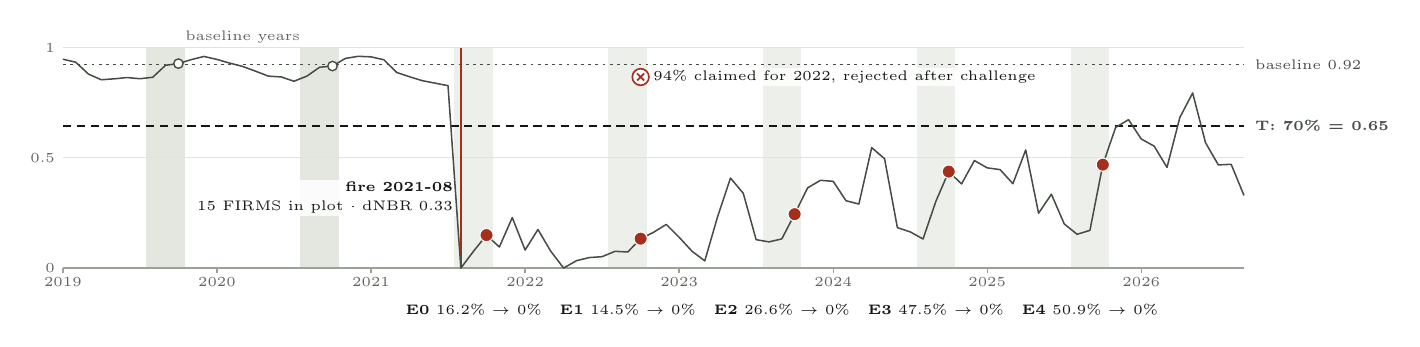
\begin{tikzpicture}[x=1cm,y=1cm]
\fill[bandbase] (1.060,0) rectangle (1.549,2.800);
\fill[bandbase] (3.016,0) rectangle (3.505,2.800);
\fill[bandepoch] (4.973,0) rectangle (5.462,2.800);
\fill[bandepoch] (6.929,0) rectangle (7.418,2.800);
\fill[bandepoch] (8.886,0) rectangle (9.375,2.800);
\fill[bandepoch] (10.842,0) rectangle (11.332,2.800);
\fill[bandepoch] (12.799,0) rectangle (13.288,2.800);
\draw[grid] (0,1.400) -- (15.000,1.400);
\draw[grid] (0,2.800) -- (15.000,2.800);
\draw[axis] (0,0) -- (15.000,0);
\node[ticklabel, anchor=east] at (-0.06,0.000) {0};
\node[ticklabel, anchor=east] at (-0.06,1.400) {0.5};
\node[ticklabel, anchor=east] at (-0.06,2.800) {1};
\draw[axis] (0.000,0) -- (0.000,-0.06);
\node[ticklabel, anchor=north] at (0.000,-0.08) {2019};
\draw[axis] (1.957,0) -- (1.957,-0.06);
\node[ticklabel, anchor=north] at (1.957,-0.08) {2020};
\draw[axis] (3.913,0) -- (3.913,-0.06);
\node[ticklabel, anchor=north] at (3.913,-0.08) {2021};
\draw[axis] (5.870,0) -- (5.870,-0.06);
\node[ticklabel, anchor=north] at (5.870,-0.08) {2022};
\draw[axis] (7.826,0) -- (7.826,-0.06);
\node[ticklabel, anchor=north] at (7.826,-0.08) {2023};
\draw[axis] (9.783,0) -- (9.783,-0.06);
\node[ticklabel, anchor=north] at (9.783,-0.08) {2024};
\draw[axis] (11.739,0) -- (11.739,-0.06);
\node[ticklabel, anchor=north] at (11.739,-0.08) {2025};
\draw[axis] (13.696,0) -- (13.696,-0.06);
\node[ticklabel, anchor=north] at (13.696,-0.08) {2026};
\node[ticklabel, anchor=south] at (2.283,2.820) {baseline years};
\draw[baseline] (0,2.582) -- (15.000,2.582);
\draw[threshold] (0,1.807) -- (15.000,1.807);
\node[sidelabel] at (15.100,2.582) {baseline 0.92};
\node[sidelabel, font=\tiny\bfseries] at (15.100,1.807) {T: 70\% = 0.65};
\draw[fire] (5.054,0) -- (5.054,2.800);
\node[annot, anchor=east, align=right] at (4.994,0.896) {\textbf{fire 2021-08}\\15 FIRMS in plot · dNBR 0.33};
\draw[series] (0.000,2.653) -- (0.163,2.615) -- (0.326,2.463) -- (0.489,2.392) -- (0.652,2.404) -- (0.815,2.420) -- (0.978,2.405) -- (1.141,2.424) -- (1.304,2.576) -- (1.467,2.597) -- (1.630,2.648) -- (1.793,2.688) -- (1.957,2.650) -- (2.120,2.603) -- (2.283,2.561) -- (2.446,2.501) -- (2.609,2.438) -- (2.772,2.428) -- (2.935,2.373) -- (3.098,2.438) -- (3.261,2.551) -- (3.424,2.566) -- (3.587,2.663) -- (3.750,2.690) -- (3.913,2.683) -- (4.076,2.646) -- (4.239,2.485) -- (4.402,2.430) -- (4.565,2.380) -- (4.728,2.349) -- (4.891,2.317) -- (5.054,0.000) -- (5.217,0.217) -- (5.380,0.419) -- (5.543,0.268) -- (5.707,0.642) -- (5.870,0.230) -- (6.033,0.490) -- (6.196,0.214) -- (6.359,0.001) -- (6.522,0.094) -- (6.685,0.134) -- (6.848,0.145) -- (7.011,0.213) -- (7.174,0.205) -- (7.337,0.374) -- (7.500,0.454) -- (7.663,0.555) -- (7.826,0.392) -- (7.989,0.215) -- (8.152,0.092) -- (8.315,0.654) -- (8.478,1.144) -- (8.641,0.949) -- (8.804,0.361) -- (8.967,0.333) -- (9.130,0.371) -- (9.293,0.685) -- (9.457,1.018) -- (9.620,1.115) -- (9.783,1.102) -- (9.946,0.855) -- (10.109,0.814) -- (10.272,1.530) -- (10.435,1.389) -- (10.598,0.514) -- (10.761,0.460) -- (10.924,0.370) -- (11.087,0.849) -- (11.250,1.226) -- (11.413,1.069) -- (11.576,1.366) -- (11.739,1.273) -- (11.902,1.251) -- (12.065,1.072) -- (12.228,1.501) -- (12.391,0.697) -- (12.554,0.938) -- (12.717,0.561) -- (12.880,0.430) -- (13.043,0.479) -- (13.207,1.314) -- (13.370,1.787) -- (13.533,1.885) -- (13.696,1.639) -- (13.859,1.549) -- (14.022,1.279) -- (14.185,1.913) -- (14.348,2.224) -- (14.511,1.593) -- (14.674,1.311) -- (14.837,1.318) -- (15.000,0.923);
\node[basepoint] at (1.467,2.597) {};
\node[basepoint] at (3.424,2.566) {};
\node[scored, fill=critical] at (5.380,0.419) {};
\node[scored, fill=critical] at (7.337,0.374) {};
\node[scored, fill=critical] at (9.293,0.685) {};
\node[scored, fill=critical] at (11.250,1.226) {};
\node[scored, fill=critical] at (13.207,1.314) {};
\node[rejected] at (7.337,2.427) {};
\draw[critical, line width=0.6pt] (7.292,2.382) -- (7.382,2.472) (7.292,2.472) -- (7.382,2.382);
\node[annot, anchor=west] at (7.457,2.427) {94\% claimed for 2022, rejected after challenge};
\node[epochlabel] at (5.217,-0.42) {\textbf{E0} 16.2\% $\rightarrow$ 0\%};
\node[epochlabel] at (7.174,-0.42) {\textbf{E1} 14.5\% $\rightarrow$ 0\%};
\node[epochlabel] at (9.130,-0.42) {\textbf{E2} 26.6\% $\rightarrow$ 0\%};
\node[epochlabel] at (11.087,-0.42) {\textbf{E3} 47.5\% $\rightarrow$ 0\%};
\node[epochlabel] at (13.043,-0.42) {\textbf{E4} 50.9\% $\rightarrow$ 0\%};
\end{tikzpicture}


\figcaption{Monthly canopy fraction of each 250\,ha plot (line; gaps are cloudy months). Shaded: the scored
Aug--Oct seasons, darker for the baseline years. Dots: the month each year was scored on, coloured by outcome;
hollow dots: baseline months. At Yedigöller the winter dips are leaf-off broadleaf trees and low sun; that and clouds are why only Aug--Oct is scored. Under each
year: canopy retained $\rightarrow$ share of that tranche released.}

\vspace{2pt}
\textbf{What the series show.} The Manavgat fire is confirmed three independent ways: canopy falls from \FireBefore\ to
\FireAfter\ in \FireMonth, the burn ratio drops by dNBR \FireDnbr, and \FireFirms\ NASA FIRMS detections
fall inside the plot on \FireFirst\ and \FireLast. Over the Amazon plot, a September 2022 reading falls from
\SmokeBefore\ to \SmokeAfter\ while NBR holds at \SmokeNbr\ and the canopy is back the next season: haze, which is why each
year is scored on its greenest month rather than its mean. The September 2024 drop there does carry a burn signature
(dNBR \NovoFireDnbr, \NovoFireFirms\ FIRMS detections in plot) and is recorded in that year's evidence.

\newpage
% =================================================================================== page 4
\sect{08}{Why this needs a chain}
{\small
\renewcommand{\arraystretch}{1.12}
\begin{tabularx}{\textwidth}{@{}>{\raggedright\arraybackslash}p{3.5cm}X@{}}
\textbf{Why not a database?} & Its owner is always one of the three parties: funder, developer or verifier. Here nobody
has to own the ledger, and a plot's identity is unique across everyone who uses it.\\
\textbf{Why not an escrow agent?} & Escrow can lock money, but not the number that unlocks it: whoever computes survival
controls the payment. Here the computation is reproducible from hashed evidence and the reporter is staked.\\
\textbf{Why not just signatures?} & A signature shows who said something. It does not stop them from saying two
different things, and lying costs nothing. One live claim per plot-year, a stake behind it and a public challenge
window make a false claim visible and expensive.\\
\textbf{Is the measurement on chain?} & No, and we do not pretend it is. The chain holds the economic game and the
evidence hashes; anyone can rerun the method on the same series and get the same number, as the Verify page does.\\
\end{tabularx}}

\sect{09}{Who uses it, and how it gets adopted}
\begin{minipage}[t]{0.48\textwidth}\raggedright
\textbf{Users}
\begin{itemize}
  \item \textbf{Funders and credit buyers} (corporate pre-purchase, climate funds) paying for outcomes, not promises.
  \item \textbf{Project developers} raising staged money against a credible, public survival record.
  \item \textbf{Independent verifiers} who earn by staking on accurate claims and lose stake on wrong ones.
  \item \textbf{Registries} that need a guard against the same land being registered twice.
\end{itemize}
\end{minipage}\hfill
\begin{minipage}[t]{0.48\textwidth}\raggedright
\textbf{Adoption path}
\begin{enumerate}
  \item Run beside an existing project as a monitoring layer; its carbon methodology is untouched.
  \item A funder escrows one pilot tranche against the project's real boundary.
  \item Open the verifier role to staked third parties; challengers keep them honest.
  \item Replace the single arbiter with a multisig or dispute protocol; add radar or lidar so canopy
        \emph{structure}, not only greenness, is measured.
\end{enumerate}
\end{minipage}

\sect{10}{Cost and scale}
\begin{minipage}[t]{0.47\textwidth}
\vspace{0pt}
{\footnotesize
\renewcommand{\arraystretch}{1.15}
\begin{tabularx}{\linewidth}{@{}Xr@{}}
\toprule
\textbf{Action (Base Sepolia run)} & \textbf{Gas}\\
\midrule
register a plot (21--22 H3 cells) & \mono{783,214}\\
fund the escrow & \mono{78,658}\\
stake & \mono{44,998}\\
attest one plot-year & \mono{179,988}\\
finalize & \mono{41,837}\\
release one tranche & \mono{100,256}\\
challenge / resolve & \mono{118,602} / \mono{68,150}\\
\midrule
\textbf{settle one plot-year} (attest + finalize + release) & \mono{\textbf{322,081}}\\
\bottomrule
\end{tabularx}}
\end{minipage}\hfill
\begin{minipage}[t]{0.49\textwidth}\raggedright
\vspace{0pt}
\begin{itemize}
  \item \textbf{Data:} one API request returns a plot's whole \SeriesMonths-month history; three plots take
        about 40\,s on the free Copernicus tier.
  \item \textbf{Chain:} a plot costs one registration and three cheap calls a year; registration grows with the
        plot's cell count (one storage slot per H3 cell).
  \item \textbf{Double counting:} H3 is a global grid, so ``has this land already been claimed?'' is a lookup, for any
        registry that reads the contract.
\end{itemize}
\end{minipage}

\sect{11}{Limits, stated plainly}
\begin{itemize}
  \item Disputes are decided by one arbiter address in this version; production needs a multisig or dispute protocol.
  \item NDVI sees the canopy surface. Thinning under a closed canopy barely moves it, and shrub regrowth counts once its
        NDVI passes 0.5: part of Manavgat's climb to \MaxBurned\ by 2025 is maquis, not pine. The 70\% threshold keeps
        that from releasing money.
  \item Scoring on the greenest month means a loss after it is counted the following year (the September 2024 burn at
        Novo Progresso falls after that year's August score).
  \item Plots are 250\,ha squares placed by our scan, standing in for real project boundaries.
\end{itemize}

\sect{12}{Deployment, reproduction and sources}
{\footnotesize
\begin{minipage}[t]{0.5\textwidth}
\vspace{0pt}
\textbf{Base Sepolia} (chain 84532), sources verified on Sourcify\\[2pt]
\renewcommand{\arraystretch}{1.1}
\begin{tabular}{@{}ll@{}}
\mono{ProjectRegistry} & \link{https://sepolia.basescan.org/address/0x9b63be2BC0c7a056606A46cdC2Dd0cb5723fda2d}{\mono{0x9b63…da2d}}\\
\mono{SurvivalOracle} & \link{https://sepolia.basescan.org/address/0x5BA5da334254FBbDF611ad1b2AbC7B22aFB44702}{\mono{0x5BA5…4702}}\\
\mono{MilestoneEscrow} & \link{https://sepolia.basescan.org/address/0xb2AC9d36301cA0Cd1F001A19CE600fc5d6954a39}{\mono{0xb2AC…4a39}}\\
\end{tabular}\\[3pt]
Every transaction of the run: \mono{deployments/84532.demo.json} and each plot's page on the site.
\end{minipage}\hfill
\begin{minipage}[t]{0.47\textwidth}
\vspace{0pt}
\textbf{Reproduce}\\[2pt]
\mono{npm test}\hfill 41 Foundry tests\\
\mono{npm run oracle}\hfill Sentinel-2 + FIRMS $\rightarrow$ evidence\\
\mono{npm run demo:local}\hfill whole story on a local chain\\
\mono{npm run demo:testnet}\hfill deploy and run on Base Sepolia
\end{minipage}

\vspace{6pt}
\color{ink3}Contains modified Copernicus Sentinel data (2019--2026) via the Copernicus Data Space Ecosystem. Fires: NASA
FIRMS, VIIRS S-NPP. Site basemap: Sentinel-2 cloudless by EOX. Fonts: Instrument Sans, IBM Plex Mono (SIL OFL).}

\end{document}
